

\tikzset{every picture/.style={line width=0.75pt}} %set default line width to 0.75pt        

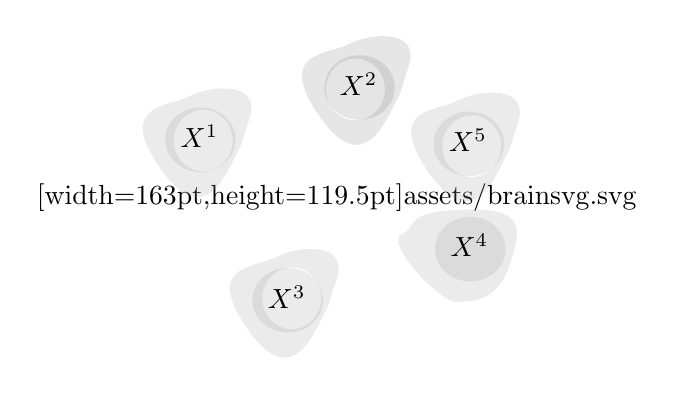
\begin{tikzpicture}[x=0.75pt,y=0.75pt,yscale=-1,xscale=1]
%uncomment if require: \path (0,293); %set diagram left start at 0, and has height of 293

%Image [id:dp7777581298700516] 
\draw (151.33,97) node   {\includesvg[width=163pt,height=119.5pt]{assets/brainsvg.svg}};
%Shape: Polygon Curved [id:ds34961065781940404] 
\draw  [draw opacity=0][fill={rgb, 255:red, 128; green, 128; blue, 128 }  ,fill opacity=0.2 ] (157.33,22.83) .. controls (167.33,17.5) and (192,15.5) .. (186,33.5) .. controls (180,51.5) and (184.67,40.83) .. (178.67,52.83) .. controls (172.67,64.83) and (162,86.17) .. (142,56.17) .. controls (122,26.17) and (147.33,28.17) .. (157.33,22.83) -- cycle ;

%Shape: Polygon Curved [id:ds12005288403924697] 
\draw  [draw opacity=0][fill={rgb, 255:red, 155; green, 155; blue, 155 }  ,fill opacity=0.2 ] (122.67,125.33) .. controls (132.67,120) and (157.33,118) .. (151.33,136) .. controls (145.33,154) and (150,143.33) .. (144,155.33) .. controls (138,167.33) and (127.33,188.67) .. (107.33,158.67) .. controls (87.33,128.67) and (112.67,130.67) .. (122.67,125.33) -- cycle ;

%Shape: Polygon Curved [id:ds2775692663684084] 
\draw  [draw opacity=0][fill={rgb, 255:red, 155; green, 155; blue, 155 }  ,fill opacity=0.2 ] (210,50) .. controls (220,44.67) and (244.67,42.67) .. (238.67,60.67) .. controls (232.67,78.67) and (237.33,68) .. (231.33,80) .. controls (225.33,92) and (214.67,113.33) .. (194.67,83.33) .. controls (174.67,53.33) and (200,55.33) .. (210,50) -- cycle ;

%Shape: Polygon Curved [id:ds2694891835945543] 
\draw  [draw opacity=0][fill={rgb, 255:red, 155; green, 155; blue, 155 }  ,fill opacity=0.2 ] (80.67,48) .. controls (90.67,42.67) and (115.33,40.67) .. (109.33,58.67) .. controls (103.33,76.67) and (108,66) .. (102,78) .. controls (96,90) and (85.33,111.33) .. (65.33,81.33) .. controls (45.33,51.33) and (70.67,53.33) .. (80.67,48) -- cycle ;

%Shape: Ellipse [id:dp22575039289402277] 
\draw  [color={rgb, 255:red, 255; green, 255; blue, 255 }  ,draw opacity=1 ][fill={rgb, 255:red, 255; green, 255; blue, 255 }  ,fill opacity=1 ] (73.33,69.4) .. controls (73.33,61.48) and (79.45,55.07) .. (87,55.07) .. controls (94.55,55.07) and (100.67,61.48) .. (100.67,69.4) .. controls (100.67,77.32) and (94.55,83.73) .. (87,83.73) .. controls (79.45,83.73) and (73.33,77.32) .. (73.33,69.4) -- cycle ;
%Shape: Ellipse [id:dp3623945699685074] 
\draw  [color={rgb, 255:red, 255; green, 255; blue, 255 }  ,draw opacity=1 ][fill={rgb, 255:red, 255; green, 255; blue, 255 }  ,fill opacity=1 ] (116,145.4) .. controls (116,137.48) and (122.12,131.07) .. (129.67,131.07) .. controls (137.21,131.07) and (143.33,137.48) .. (143.33,145.4) .. controls (143.33,153.32) and (137.21,159.73) .. (129.67,159.73) .. controls (122.12,159.73) and (116,153.32) .. (116,145.4) -- cycle ;
%Shape: Ellipse [id:dp4899964637813463] 
\draw  [color={rgb, 255:red, 255; green, 255; blue, 255 }  ,draw opacity=1 ][fill={rgb, 255:red, 255; green, 255; blue, 255 }  ,fill opacity=1 ] (146.67,44.73) .. controls (146.67,36.82) and (152.79,30.4) .. (160.33,30.4) .. controls (167.88,30.4) and (174,36.82) .. (174,44.73) .. controls (174,52.65) and (167.88,59.07) .. (160.33,59.07) .. controls (152.79,59.07) and (146.67,52.65) .. (146.67,44.73) -- cycle ;
%Shape: Ellipse [id:dp8906821910938405] 
\draw  [color={rgb, 255:red, 255; green, 255; blue, 255 }  ,draw opacity=1 ][fill={rgb, 255:red, 255; green, 255; blue, 255 }  ,fill opacity=1 ] (202.67,72.07) .. controls (202.67,64.15) and (208.79,57.73) .. (216.33,57.73) .. controls (223.88,57.73) and (230,64.15) .. (230,72.07) .. controls (230,79.98) and (223.88,86.4) .. (216.33,86.4) .. controls (208.79,86.4) and (202.67,79.98) .. (202.67,72.07) -- cycle ;
%Shape: Ellipse [id:dp1843235766479494] 
\draw  [color={rgb, 255:red, 255; green, 255; blue, 255 }  ,draw opacity=1 ][fill={rgb, 255:red, 255; green, 255; blue, 255 }  ,fill opacity=1 ] (200,122.73) .. controls (200,114.82) and (206.12,108.4) .. (213.67,108.4) .. controls (221.21,108.4) and (227.33,114.82) .. (227.33,122.73) .. controls (227.33,130.65) and (221.21,137.07) .. (213.67,137.07) .. controls (206.12,137.07) and (200,130.65) .. (200,122.73) -- cycle ;
%Shape: Polygon Curved [id:ds6576330285171925] 
\draw  [draw opacity=0][fill={rgb, 255:red, 155; green, 155; blue, 155 }  ,fill opacity=0.2 ] (212,102.67) .. controls (242,101.47) and (240.67,111.2) .. (234.67,129.2) .. controls (228.67,147.2) and (217.33,146.53) .. (209.33,147.2) .. controls (201.33,147.87) and (174,118.4) .. (182.67,114.53) .. controls (191.33,110.67) and (182,103.87) .. (212,102.67) -- cycle ;


% Text Node
\draw  [draw opacity=0][fill={rgb, 255:red, 128; green, 128; blue, 128 }  ,fill opacity=0.2 ]  (162.33, 43.83) circle [x radius= 16.97, y radius= 15.56]   ;
\draw (151.33,35.23) node [anchor=north west][inner sep=0.75pt]    {$X^{2}$};
% Text Node
\draw  [draw opacity=0][fill={rgb, 255:red, 155; green, 155; blue, 155 }  ,fill opacity=0.2 ]  (127.67, 146.33) circle [x radius= 16.97, y radius= 15.56]   ;
\draw (116.67,137.73) node [anchor=north west][inner sep=0.75pt]    {$X^{3}$};
% Text Node
\draw  [draw opacity=0][fill={rgb, 255:red, 155; green, 155; blue, 155 }  ,fill opacity=0.2 ]  (215, 71) circle [x radius= 16.97, y radius= 15.56]   ;
\draw (204,62.4) node [anchor=north west][inner sep=0.75pt]    {$X^{5}$};
% Text Node
\draw  [draw opacity=0][fill={rgb, 255:red, 155; green, 155; blue, 155 }  ,fill opacity=0.2 ]  (85.67, 69) circle [x radius= 16.97, y radius= 15.56]   ;
\draw (74.67,60.4) node [anchor=north west][inner sep=0.75pt]    {$X^{1}$};
% Text Node
\draw  [draw opacity=0][fill={rgb, 255:red, 155; green, 155; blue, 155 }  ,fill opacity=0.2 ]  (215.67, 121.67) circle [x radius= 16.97, y radius= 15.56]   ;
\draw (204.67,113.07) node [anchor=north west][inner sep=0.75pt]    {$X^{4}$};


\end{tikzpicture}
